\documentclass[1p]{elsarticle_modified}
%\bibliographystyle{elsarticle-num}

%\usepackage[colorlinks]{hyperref}
%\usepackage{abbrmath_seonhwa} %\Abb, \Ascr, \Acal ,\Abf, \Afrak
\usepackage{amsfonts}
\usepackage{amssymb}
\usepackage{amsmath}
\usepackage{amsthm}
\usepackage{scalefnt}
\usepackage{amsbsy}
\usepackage{kotex}
\usepackage{caption}
\usepackage{subfig}
\usepackage{color}
\usepackage{graphicx}
\usepackage{xcolor} %% white, black, red, green, blue, cyan, magenta, yellow
\usepackage{float}
\usepackage{setspace}
\usepackage{hyperref}

\usepackage{tikz}
\usetikzlibrary{arrows}

\usepackage{multirow}
\usepackage{array} % fixed length table
\usepackage{hhline}

%%%%%%%%%%%%%%%%%%%%%
\makeatletter
\renewcommand*\env@matrix[1][\arraystretch]{%
	\edef\arraystretch{#1}%
	\hskip -\arraycolsep
	\let\@ifnextchar\new@ifnextchar
	\array{*\c@MaxMatrixCols c}}
\makeatother %https://tex.stackexchange.com/questions/14071/how-can-i-increase-the-line-spacing-in-a-matrix
%%%%%%%%%%%%%%%

\usepackage[normalem]{ulem}

\newcommand{\msout}[1]{\ifmmode\text{\sout{\ensuremath{#1}}}\else\sout{#1}\fi}
%SOURCE: \msout is \stkout macro in https://tex.stackexchange.com/questions/20609/strikeout-in-math-mode

\newcommand{\cancel}[1]{
	\ifmmode
	{\color{red}\msout{#1}}
	\else
	{\color{red}\sout{#1}}
	\fi
}

\newcommand{\add}[1]{
	{\color{blue}\uwave{#1}}
}

\newcommand{\replace}[2]{
	\ifmmode
	{\color{red}\msout{#1}}{\color{blue}\uwave{#2}}
	\else
	{\color{red}\sout{#1}}{\color{blue}\uwave{#2}}
	\fi
}

\newcommand{\Sol}{\mathcal{S}} %segment
\newcommand{\D}{D} %diagram
\newcommand{\A}{\mathcal{A}} %arc


%%%%%%%%%%%%%%%%%%%%%%%%%%%%%5 test

\def\sl{\operatorname{\textup{SL}}(2,\Cbb)}
\def\psl{\operatorname{\textup{PSL}}(2,\Cbb)}
\def\quan{\mkern 1mu \triangleright \mkern 1mu}

\theoremstyle{definition}
\newtheorem{thm}{Theorem}[section]
\newtheorem{prop}[thm]{Proposition}
\newtheorem{lem}[thm]{Lemma}
\newtheorem{ques}[thm]{Question}
\newtheorem{cor}[thm]{Corollary}
\newtheorem{defn}[thm]{Definition}
\newtheorem{exam}[thm]{Example}
\newtheorem{rmk}[thm]{Remark}
\newtheorem{alg}[thm]{Algorithm}

\newcommand{\I}{\sqrt{-1}}
\begin{document}

%\begin{frontmatter}
%
%\title{Boundary parabolic representations of knots up to 8 crossings}
%
%%% Group authors per affiliation:
%\author{Yunhi Cho} 
%\address{Department of Mathematics, University of Seoul, Seoul, Korea}
%\ead{yhcho@uos.ac.kr}
%
%
%\author{Seonhwa Kim} %\fnref{s_kim}}
%\address{Center for Geometry and Physics, Institute for Basic Science, Pohang, 37673, Korea}
%\ead{ryeona17@ibs.re.kr}
%
%\author{Hyuk Kim}
%\address{Department of Mathematical Sciences, Seoul National University, Seoul 08826, Korea}
%\ead{hyukkim@snu.ac.kr}
%
%\author{Seokbeom Yoon}
%\address{Department of Mathematical Sciences, Seoul National University, Seoul, 08826,  Korea}
%\ead{sbyoon15@snu.ac.kr}
%
%\begin{abstract}
%We find all boundary parabolic representation of knots up to 8 crossings.
%
%\end{abstract}
%\begin{keyword}
%    \MSC[2010] 57M25 
%\end{keyword}
%
%\end{frontmatter}

%\linenumbers
%\tableofcontents
%
\newcommand\colored[1]{\textcolor{white}{\rule[-0.35ex]{0.8em}{1.4ex}}\kern-0.8em\color{red} #1}%
%\newcommand\colored[1]{\textcolor{white}{ #1}\kern-2.17ex	\textcolor{white}{ #1}\kern-1.81ex	\textcolor{white}{ #1}\kern-2.15ex\color{red}#1	}

{\Large $\underline{11n_{117}~(K11n_{117})}$}

\setlength{\tabcolsep}{10pt}
\renewcommand{\arraystretch}{1.6}
\vspace{1cm}\begin{tabular}{m{100pt}>{\centering\arraybackslash}m{274pt}}
\multirow{5}{120pt}{
	\centering
	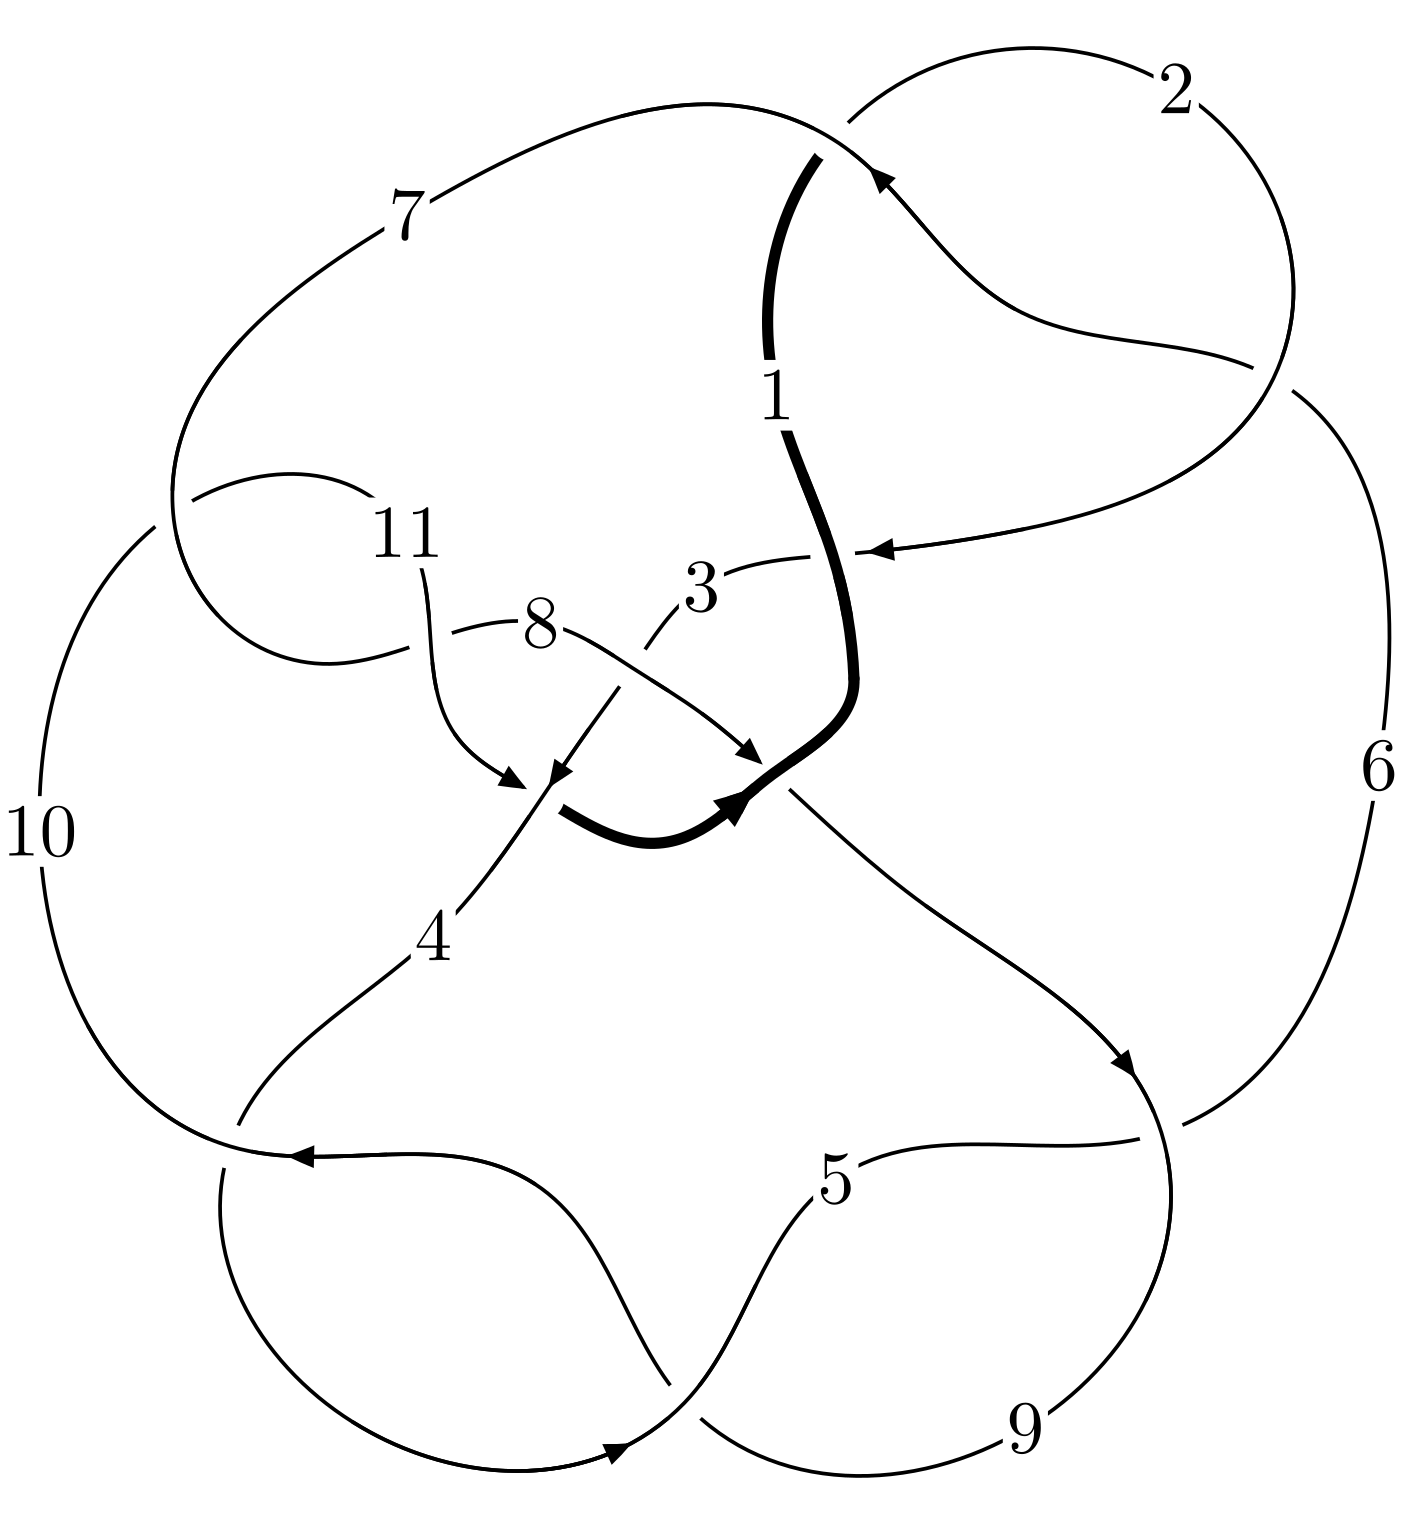
\includegraphics[width=112pt]{../../../GIT/diagram.site/Diagrams/png/733_11n_117.png}\\
\ \ \ A knot diagram\footnotemark}&
\allowdisplaybreaks
\textbf{Linearized knot diagam} \\
\cline{2-2}
 &
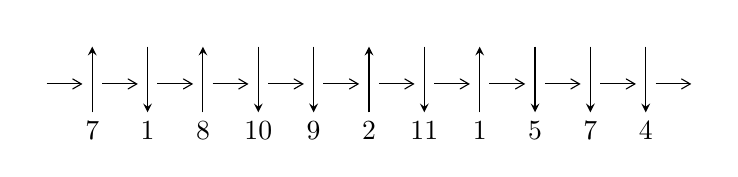
\begin{tikzpicture}[x=20pt, y=17pt]
	% nodes
	\node (C0) at (0, 0) {};
	\node (C1) at (1, 0) {};
	\node (C1U) at (1, +1) {};
	\node (C1D) at (1, -1) {7};

	\node (C2) at (2, 0) {};
	\node (C2U) at (2, +1) {};
	\node (C2D) at (2, -1) {1};

	\node (C3) at (3, 0) {};
	\node (C3U) at (3, +1) {};
	\node (C3D) at (3, -1) {8};

	\node (C4) at (4, 0) {};
	\node (C4U) at (4, +1) {};
	\node (C4D) at (4, -1) {10};

	\node (C5) at (5, 0) {};
	\node (C5U) at (5, +1) {};
	\node (C5D) at (5, -1) {9};

	\node (C6) at (6, 0) {};
	\node (C6U) at (6, +1) {};
	\node (C6D) at (6, -1) {2};

	\node (C7) at (7, 0) {};
	\node (C7U) at (7, +1) {};
	\node (C7D) at (7, -1) {11};

	\node (C8) at (8, 0) {};
	\node (C8U) at (8, +1) {};
	\node (C8D) at (8, -1) {1};

	\node (C9) at (9, 0) {};
	\node (C9U) at (9, +1) {};
	\node (C9D) at (9, -1) {5};

	\node (C10) at (10, 0) {};
	\node (C10U) at (10, +1) {};
	\node (C10D) at (10, -1) {7};

	\node (C11) at (11, 0) {};
	\node (C11U) at (11, +1) {};
	\node (C11D) at (11, -1) {4};
	\node (C12) at (12, 0) {};

	% arrows
	\draw[->,>={angle 60}]
	(C0) edge (C1) (C1) edge (C2) (C2) edge (C3) (C3) edge (C4) (C4) edge (C5) (C5) edge (C6) (C6) edge (C7) (C7) edge (C8) (C8) edge (C9) (C9) edge (C10) (C10) edge (C11) (C11) edge (C12) ;	\draw[->,>=stealth]
	(C1D) edge (C1U) (C2U) edge (C2D) (C3D) edge (C3U) (C4U) edge (C4D) (C5U) edge (C5D) (C6D) edge (C6U) (C7U) edge (C7D) (C8D) edge (C8U) (C9U) edge (C9D) (C10U) edge (C10D) (C11U) edge (C11D) ;
	\end{tikzpicture} \\
\hhline{~~} \\& 
\textbf{Solving Sequence} \\ \cline{2-2} 
 &
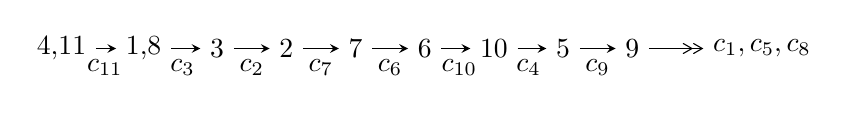
\begin{tikzpicture}[x=25pt, y=7pt]
	% node
	\node (A0) at (-1/8, 0) {4,11};
	\node (A1) at (17/16, 0) {1,8};
	\node (A2) at (17/8, 0) {3};
	\node (A3) at (25/8, 0) {2};
	\node (A4) at (33/8, 0) {7};
	\node (A5) at (41/8, 0) {6};
	\node (A6) at (49/8, 0) {10};
	\node (A7) at (57/8, 0) {5};
	\node (A8) at (65/8, 0) {9};
	\node (C1) at (1/2, -1) {$c_{11}$};
	\node (C2) at (13/8, -1) {$c_{3}$};
	\node (C3) at (21/8, -1) {$c_{2}$};
	\node (C4) at (29/8, -1) {$c_{7}$};
	\node (C5) at (37/8, -1) {$c_{6}$};
	\node (C6) at (45/8, -1) {$c_{10}$};
	\node (C7) at (53/8, -1) {$c_{4}$};
	\node (C8) at (61/8, -1) {$c_{9}$};
	\node (A9) at (10, 0) {$c_{1},c_{5},c_{8}$};

	% edge
	\draw[->,>=stealth]	
	(A0) edge (A1) (A1) edge (A2) (A2) edge (A3) (A3) edge (A4) (A4) edge (A5) (A5) edge (A6) (A6) edge (A7) (A7) edge (A8) ;
	\draw[->>,>={angle 60}]	
	(A8) edge (A9);
\end{tikzpicture} \\ 

\end{tabular} \\

\footnotetext{
The image of knot diagram is generated by the software ``\textbf{Draw programme}" developed by Andrew Bartholomew(\url{http://www.layer8.co.uk/maths/draw/index.htm\#Running-draw}), where we modified some parts for our purpose(\url{https://github.com/CATsTAILs/LinksPainter}).
}\phantom \\ \newline 
\centering \textbf{Ideals for irreducible components\footnotemark of $X_{\text{par}}$} 
 
\begin{align*}
I^u_{1}&=\langle 
7 u^{12}+50 u^{11}+\cdots+2 b+42,\;7 u^{12}+54 u^{11}+\cdots+4 a+52,\\
\phantom{I^u_{1}}&\phantom{= \langle  }u^{13}+8 u^{12}+33 u^{11}+88 u^{10}+170 u^9+251 u^8+292 u^7+262 u^6+172 u^5+79 u^4+38 u^3+31 u^2+18 u+4\rangle \\
I^u_{2}&=\langle 
-3 a^3 u^2+2 a^3 u+2 a^2 u^2+4 a^3-3 a^2 u-5 u^2 a- a^2+3 u^2+5 b+10 a-7 u+6,\\
\phantom{I^u_{2}}&\phantom{= \langle  }a^4- a^3 u+3 a^2 u^2-5 a^2 u+5 a^2- a u+8 u^2+a-15 u+11,\;u^3- u^2+1\rangle \\
I^u_{3}&=\langle 
u^7-2 u^6+3 u^5-2 u^4-2 u^3+3 u^2+b- u-1,\;u^5-2 u^4+4 u^3-4 u^2+a+2 u,\\
\phantom{I^u_{3}}&\phantom{= \langle  }u^8-3 u^7+6 u^6-7 u^5+4 u^4+u^3-2 u^2+1\rangle \\
\\
\end{align*}
\raggedright * 3 irreducible components of $\dim_{\mathbb{C}}=0$, with total 33 representations.\\
\footnotetext{All coefficients of polynomials are rational numbers. But the coefficients are sometimes approximated in decimal forms when there is not enough margin.}
\newpage
\renewcommand{\arraystretch}{1}
\centering \section*{I. $I^u_{1}= \langle 7 u^{12}+50 u^{11}+\cdots+2 b+42,\;7 u^{12}+54 u^{11}+\cdots+4 a+52,\;u^{13}+8 u^{12}+\cdots+18 u+4 \rangle$}
\flushleft \textbf{(i) Arc colorings}\\
\begin{tabular}{m{7pt} m{180pt} m{7pt} m{180pt} }
\flushright $a_{4}=$&$\begin{pmatrix}0\\u\end{pmatrix}$ \\
\flushright $a_{11}=$&$\begin{pmatrix}1\\0\end{pmatrix}$ \\
\flushright $a_{1}=$&$\begin{pmatrix}1\\u^2\end{pmatrix}$ \\
\flushright $a_{8}=$&$\begin{pmatrix}-\frac{7}{4} u^{12}-\frac{27}{2} u^{11}+\cdots-\frac{153}{4} u-13\\-\frac{7}{2} u^{12}-25 u^{11}+\cdots-\frac{121}{2} u-21\end{pmatrix}$ \\
\flushright $a_{3}=$&$\begin{pmatrix}-\frac{1}{2} u^{12}-\frac{7}{2} u^{11}+\cdots-\frac{9}{2} u-\frac{1}{2}\\\frac{1}{2} u^{12}+3 u^{11}+\cdots+4 u^2+\frac{3}{2} u\end{pmatrix}$ \\
\flushright $a_{2}=$&$\begin{pmatrix}\frac{1}{2} u^{11}+3 u^{10}+\cdots+4 u+\frac{3}{2}\\-\frac{1}{2} u^{12}-3 u^{11}+\cdots-3 u^2-\frac{1}{2} u\end{pmatrix}$ \\
\flushright $a_{7}=$&$\begin{pmatrix}-\frac{21}{4} u^{12}-\frac{77}{2} u^{11}+\cdots-\frac{395}{4} u-34\\-\frac{7}{2} u^{12}-25 u^{11}+\cdots-\frac{121}{2} u-21\end{pmatrix}$ \\
\flushright $a_{6}=$&$\begin{pmatrix}-6 u^{12}-\frac{91}{2} u^{11}+\cdots-113 u-\frac{75}{2}\\-\frac{3}{2} u^{12}-17 u^{11}+\cdots-\frac{149}{2} u-26\end{pmatrix}$ \\
\flushright $a_{10}=$&$\begin{pmatrix}-\frac{3}{2} u^{12}-\frac{21}{2} u^{11}+\cdots-\frac{35}{2} u-\frac{9}{2}\\-\frac{3}{2} u^{12}-11 u^{11}+\cdots-\frac{43}{2} u-6\end{pmatrix}$ \\
\flushright $a_{5}=$&$\begin{pmatrix}\frac{21}{4} u^{12}+\frac{77}{2} u^{11}+\cdots+\frac{347}{4} u+26\\\frac{9}{2} u^{12}+35 u^{11}+\cdots+\frac{181}{2} u+27\end{pmatrix}$ \\
\flushright $a_{9}=$&$\begin{pmatrix}-\frac{21}{4} u^{12}-\frac{79}{2} u^{11}+\cdots-\frac{387}{4} u-32\\-\frac{5}{2} u^{12}-23 u^{11}+\cdots-\frac{165}{2} u-29\end{pmatrix}$\\ \flushright $a_{9}=$&$\begin{pmatrix}-\frac{21}{4} u^{12}-\frac{79}{2} u^{11}+\cdots-\frac{387}{4} u-32\\-\frac{5}{2} u^{12}-23 u^{11}+\cdots-\frac{165}{2} u-29\end{pmatrix}$\\&\end{tabular}
\flushleft \textbf{(ii) Obstruction class $= -1$}\\~\\
\flushleft \textbf{(iii) Cusp Shapes $= -11 u^{12}-82 u^{11}-318 u^{10}-792 u^9-1428 u^8-1957 u^7-2100 u^6-1675 u^5-912 u^4-319 u^3-215 u^2-210 u-74$}\\~\\
\newpage\renewcommand{\arraystretch}{1}
\flushleft \textbf{(iv) u-Polynomials at the component}\newline \\
\begin{tabular}{m{50pt}|m{274pt}}
Crossings & \hspace{64pt}u-Polynomials at each crossing \\
\hline $$\begin{aligned}c_{1},c_{3},c_{6}\end{aligned}$$&$\begin{aligned}
&u^{13}+10 u^{11}+\cdots-2 u+1
\end{aligned}$\\
\hline $$\begin{aligned}c_{2}\end{aligned}$$&$\begin{aligned}
&u^{13}+20 u^{12}+\cdots+4 u-1
\end{aligned}$\\
\hline $$\begin{aligned}c_{4},c_{5},c_{9}\end{aligned}$$&$\begin{aligned}
&u^{13}+7 u^{12}+\cdots+52 u+8
\end{aligned}$\\
\hline $$\begin{aligned}c_{7},c_{10}\end{aligned}$$&$\begin{aligned}
&u^{13}+u^{12}+\cdots- u+1
\end{aligned}$\\
\hline $$\begin{aligned}c_{8}\end{aligned}$$&$\begin{aligned}
&u^{13}- u^{12}+\cdots-25 u+61
\end{aligned}$\\
\hline $$\begin{aligned}c_{11}\end{aligned}$$&$\begin{aligned}
&u^{13}-8 u^{12}+\cdots+18 u-4
\end{aligned}$\\
\hline
\end{tabular}\\~\\
\newpage\renewcommand{\arraystretch}{1}
\flushleft \textbf{(v) Riley Polynomials at the component}\newline \\
\begin{tabular}{m{50pt}|m{274pt}}
Crossings & \hspace{64pt}Riley Polynomials at each crossing \\
\hline $$\begin{aligned}c_{1},c_{3},c_{6}\end{aligned}$$&$\begin{aligned}
&y^{13}+20 y^{12}+\cdots+4 y-1
\end{aligned}$\\
\hline $$\begin{aligned}c_{2}\end{aligned}$$&$\begin{aligned}
&y^{13}-56 y^{12}+\cdots+56 y-1
\end{aligned}$\\
\hline $$\begin{aligned}c_{4},c_{5},c_{9}\end{aligned}$$&$\begin{aligned}
&y^{13}+11 y^{12}+\cdots-176 y-64
\end{aligned}$\\
\hline $$\begin{aligned}c_{7},c_{10}\end{aligned}$$&$\begin{aligned}
&y^{13}-15 y^{12}+\cdots-17 y-1
\end{aligned}$\\
\hline $$\begin{aligned}c_{8}\end{aligned}$$&$\begin{aligned}
&y^{13}+31 y^{12}+\cdots+4407 y-3721
\end{aligned}$\\
\hline $$\begin{aligned}c_{11}\end{aligned}$$&$\begin{aligned}
&y^{13}+2 y^{12}+\cdots+76 y-16
\end{aligned}$\\
\hline
\end{tabular}\\~\\
\newpage\flushleft \textbf{(vi) Complex Volumes and Cusp Shapes}
$$\begin{array}{c|c|c}  
\text{Solutions to }I^u_{1}& \I (\text{vol} + \sqrt{-1}CS) & \text{Cusp shape}\\
 \hline 
\begin{aligned}
u &= -0.679884 + 0.210052 I \\
a &= \phantom{-}0.660299 + 0.261424 I \\
b &= \phantom{-}1.156160 - 0.636682 I\end{aligned}
 & \phantom{-}2.05464 + 3.32300 I & \phantom{-}2.35472 - 0.87537 I \\ \hline\begin{aligned}
u &= -0.679884 - 0.210052 I \\
a &= \phantom{-}0.660299 - 0.261424 I \\
b &= \phantom{-}1.156160 + 0.636682 I\end{aligned}
 & \phantom{-}2.05464 - 3.32300 I & \phantom{-}2.35472 + 0.87537 I \\ \hline\begin{aligned}
u &= \phantom{-}0.134806 + 1.341750 I \\
a &= -0.549424 - 0.347392 I \\
b &= \phantom{-}0.196581 + 0.458453 I\end{aligned}
 & \phantom{-}6.25855 - 1.58741 I & \phantom{-}3.86210 + 4.96482 I \\ \hline\begin{aligned}
u &= \phantom{-}0.134806 - 1.341750 I \\
a &= -0.549424 + 0.347392 I \\
b &= \phantom{-}0.196581 - 0.458453 I\end{aligned}
 & \phantom{-}6.25855 + 1.58741 I & \phantom{-}3.86210 - 4.96482 I \\ \hline\begin{aligned}
u &= -0.594830\phantom{ +0.000000I} \\
a &= -0.764918\phantom{ +0.000000I} \\
b &= -1.12298\phantom{ +0.000000I}\end{aligned}
 & -1.85194\phantom{ +0.000000I} & -5.42920\phantom{ +0.000000I} \\ \hline\begin{aligned}
u &= \phantom{-}0.405732 + 0.430962 I \\
a &= \phantom{-}0.404293 + 0.808155 I \\
b &= \phantom{-}0.019709 - 0.363243 I\end{aligned}
 & -0.133748 - 1.066330 I & -2.25480 + 6.30909 I \\ \hline\begin{aligned}
u &= \phantom{-}0.405732 - 0.430962 I \\
a &= \phantom{-}0.404293 - 0.808155 I \\
b &= \phantom{-}0.019709 + 0.363243 I\end{aligned}
 & -0.133748 + 1.066330 I & -2.25480 - 6.30909 I \\ \hline\begin{aligned}
u &= -1.23597 + 1.03056 I \\
a &= \phantom{-}0.522817 - 1.037940 I \\
b &= -1.59018 + 0.77503 I\end{aligned}
 & -10.3151 + 11.3952 I & -4.67074 - 5.46785 I \\ \hline\begin{aligned}
u &= -1.23597 - 1.03056 I \\
a &= \phantom{-}0.522817 + 1.037940 I \\
b &= -1.59018 - 0.77503 I\end{aligned}
 & -10.3151 - 11.3952 I & -4.67074 + 5.46785 I \\ \hline\begin{aligned}
u &= -1.19711 + 1.14120 I \\
a &= -0.773854 + 0.862682 I \\
b &= \phantom{-}1.62163 - 0.33100 I\end{aligned}
 & -14.5236 + 4.3483 I & -7.04341 - 2.19507 I\\
 \hline 
 \end{array}$$\newpage$$\begin{array}{c|c|c}  
\text{Solutions to }I^u_{1}& \I (\text{vol} + \sqrt{-1}CS) & \text{Cusp shape}\\
 \hline 
\begin{aligned}
u &= -1.19711 - 1.14120 I \\
a &= -0.773854 - 0.862682 I \\
b &= \phantom{-}1.62163 + 0.33100 I\end{aligned}
 & -14.5236 - 4.3483 I & -7.04341 + 2.19507 I \\ \hline\begin{aligned}
u &= -1.13016 + 1.29050 I \\
a &= \phantom{-}0.868328 - 0.530434 I \\
b &= -1.342400 - 0.094615 I\end{aligned}
 & -9.55616 - 2.72200 I & -5.53329 + 1.17863 I \\ \hline\begin{aligned}
u &= -1.13016 - 1.29050 I \\
a &= \phantom{-}0.868328 + 0.530434 I \\
b &= -1.342400 + 0.094615 I\end{aligned}
 & -9.55616 + 2.72200 I & -5.53329 - 1.17863 I\\
 \hline 
 \end{array}$$\newpage\newpage\renewcommand{\arraystretch}{1}
\centering \section*{II. $I^u_{2}= \langle -3 a^3 u^2+2 a^2 u^2+\cdots+10 a+6,\;3 a^2 u^2+8 u^2+\cdots+a+11,\;u^3- u^2+1 \rangle$}
\flushleft \textbf{(i) Arc colorings}\\
\begin{tabular}{m{7pt} m{180pt} m{7pt} m{180pt} }
\flushright $a_{4}=$&$\begin{pmatrix}0\\u\end{pmatrix}$ \\
\flushright $a_{11}=$&$\begin{pmatrix}1\\0\end{pmatrix}$ \\
\flushright $a_{1}=$&$\begin{pmatrix}1\\u^2\end{pmatrix}$ \\
\flushright $a_{8}=$&$\begin{pmatrix}a\\\frac{3}{5} a^3 u^2-\frac{2}{5} a^2 u^2+\cdots-2 a-\frac{6}{5}\end{pmatrix}$ \\
\flushright $a_{3}=$&$\begin{pmatrix}- a^2 u\\\frac{2}{5} a^3 u^2-\frac{3}{5} a^2 u^2+\cdots- a+\frac{6}{5}\end{pmatrix}$ \\
\flushright $a_{2}=$&$\begin{pmatrix}\frac{2}{5} a^3 u^2+\frac{2}{5} a^2 u^2+\cdots- a+\frac{6}{5}\\a^3 u^2- a^3+a u+4 u^2-2 a-2 u\end{pmatrix}$ \\
\flushright $a_{7}=$&$\begin{pmatrix}\frac{3}{5} a^3 u^2-\frac{2}{5} a^2 u^2+\cdots- a-\frac{6}{5}\\\frac{3}{5} a^3 u^2-\frac{2}{5} a^2 u^2+\cdots-2 a-\frac{6}{5}\end{pmatrix}$ \\
\flushright $a_{6}=$&$\begin{pmatrix}-\frac{3}{5} a^3 u^2+\frac{2}{5} a^2 u^2+\cdots+a+\frac{6}{5}\\a^3 u^2+2 a^3 u+a^3-2 a^2 u+2 u^2 a+a u+4 u^2+2 a-6 u+4\end{pmatrix}$ \\
\flushright $a_{10}=$&$\begin{pmatrix}\frac{3}{5} a^3 u^2-\frac{2}{5} a^2 u^2+\cdots- a-\frac{6}{5}\\\frac{2}{5} a^3 u^2+\frac{2}{5} a^2 u^2+\cdots-2 a-\frac{4}{5}\end{pmatrix}$ \\
\flushright $a_{5}=$&$\begin{pmatrix}\frac{3}{5} a^3 u^2-\frac{2}{5} a^2 u^2+\cdots- a-\frac{6}{5}\\-\frac{3}{5} a^3 u^2+\frac{2}{5} a^2 u^2+\cdots-2 a-\frac{14}{5}\end{pmatrix}$ \\
\flushright $a_{9}=$&$\begin{pmatrix}\frac{3}{5} a^3 u^2-\frac{2}{5} a^2 u^2+\cdots- a-\frac{6}{5}\\- a^3 u- a^3+a^2 u- u^2 a- u^2-2 a+2 u-2\end{pmatrix}$\\ \flushright $a_{9}=$&$\begin{pmatrix}\frac{3}{5} a^3 u^2-\frac{2}{5} a^2 u^2+\cdots- a-\frac{6}{5}\\- a^3 u- a^3+a^2 u- u^2 a- u^2-2 a+2 u-2\end{pmatrix}$\\&\end{tabular}
\flushleft \textbf{(ii) Obstruction class $= -1$}\\~\\
\flushleft \textbf{(iii) Cusp Shapes $= -\frac{4}{5} a^3 u^2+\frac{16}{5} a^3 u-\frac{4}{5} a^2 u^2+\frac{12}{5} a^3-\frac{4}{5} a^2 u-\frac{8}{5} a^2+4 a u-\frac{16}{5} u^2+\frac{44}{5} u-\frac{42}{5}$}\\~\\
\newpage\renewcommand{\arraystretch}{1}
\flushleft \textbf{(iv) u-Polynomials at the component}\newline \\
\begin{tabular}{m{50pt}|m{274pt}}
Crossings & \hspace{64pt}u-Polynomials at each crossing \\
\hline $$\begin{aligned}c_{1},c_{3},c_{6}\end{aligned}$$&$\begin{aligned}
&u^{12}+u^{11}+\cdots-28 u+19
\end{aligned}$\\
\hline $$\begin{aligned}c_{2}\end{aligned}$$&$\begin{aligned}
&u^{12}+15 u^{11}+\cdots+1116 u+361
\end{aligned}$\\
\hline $$\begin{aligned}c_{4},c_{5},c_{9}\end{aligned}$$&$\begin{aligned}
&(u^2- u+1)^6
\end{aligned}$\\
\hline $$\begin{aligned}c_{7},c_{10}\end{aligned}$$&$\begin{aligned}
&u^{12}+3 u^{11}+\cdots+36 u+7
\end{aligned}$\\
\hline $$\begin{aligned}c_{8}\end{aligned}$$&$\begin{aligned}
&u^{12}+u^{11}+\cdots+72 u+61
\end{aligned}$\\
\hline $$\begin{aligned}c_{11}\end{aligned}$$&$\begin{aligned}
&(u^3+u^2-1)^4
\end{aligned}$\\
\hline
\end{tabular}\\~\\
\newpage\renewcommand{\arraystretch}{1}
\flushleft \textbf{(v) Riley Polynomials at the component}\newline \\
\begin{tabular}{m{50pt}|m{274pt}}
Crossings & \hspace{64pt}Riley Polynomials at each crossing \\
\hline $$\begin{aligned}c_{1},c_{3},c_{6}\end{aligned}$$&$\begin{aligned}
&y^{12}+15 y^{11}+\cdots+1116 y+361
\end{aligned}$\\
\hline $$\begin{aligned}c_{2}\end{aligned}$$&$\begin{aligned}
&y^{12}-29 y^{11}+\cdots+1501032 y+130321
\end{aligned}$\\
\hline $$\begin{aligned}c_{4},c_{5},c_{9}\end{aligned}$$&$\begin{aligned}
&(y^2+y+1)^6
\end{aligned}$\\
\hline $$\begin{aligned}c_{7},c_{10}\end{aligned}$$&$\begin{aligned}
&y^{12}-5 y^{11}+\cdots-708 y+49
\end{aligned}$\\
\hline $$\begin{aligned}c_{8}\end{aligned}$$&$\begin{aligned}
&y^{12}+23 y^{11}+\cdots-3964 y+3721
\end{aligned}$\\
\hline $$\begin{aligned}c_{11}\end{aligned}$$&$\begin{aligned}
&(y^3- y^2+2 y-1)^4
\end{aligned}$\\
\hline
\end{tabular}\\~\\
\newpage\flushleft \textbf{(vi) Complex Volumes and Cusp Shapes}
$$\begin{array}{c|c|c}  
\text{Solutions to }I^u_{2}& \I (\text{vol} + \sqrt{-1}CS) & \text{Cusp shape}\\
 \hline 
\begin{aligned}
u &= \phantom{-}0.877439 + 0.744862 I \\
a &= \phantom{-}0.666043 + 0.768482 I \\
b &= -1.68307 - 0.58734 I\end{aligned}
 & -1.91067 - 4.85801 I & -4.49024 + 6.44355 I \\ \hline\begin{aligned}
u &= \phantom{-}0.877439 + 0.744862 I \\
a &= \phantom{-}0.417746 - 1.155940 I \\
b &= \phantom{-}1.027310 + 0.598610 I\end{aligned}
 & -1.91067 - 4.85801 I & -4.49024 + 6.44355 I \\ \hline\begin{aligned}
u &= \phantom{-}0.877439 + 0.744862 I \\
a &= \phantom{-}0.337860 + 1.183260 I \\
b &= -0.993753 - 0.194653 I\end{aligned}
 & -1.91067 - 0.79824 I & -4.49024 - 0.48465 I \\ \hline\begin{aligned}
u &= \phantom{-}0.877439 + 0.744862 I \\
a &= -0.544210 - 0.050945 I \\
b &= \phantom{-}1.311880 - 0.378892 I\end{aligned}
 & -1.91067 - 0.79824 I & -4.49024 - 0.48465 I \\ \hline\begin{aligned}
u &= \phantom{-}0.877439 - 0.744862 I \\
a &= \phantom{-}0.666043 - 0.768482 I \\
b &= -1.68307 + 0.58734 I\end{aligned}
 & -1.91067 + 4.85801 I & -4.49024 - 6.44355 I \\ \hline\begin{aligned}
u &= \phantom{-}0.877439 - 0.744862 I \\
a &= \phantom{-}0.417746 + 1.155940 I \\
b &= \phantom{-}1.027310 - 0.598610 I\end{aligned}
 & -1.91067 + 4.85801 I & -4.49024 - 6.44355 I \\ \hline\begin{aligned}
u &= \phantom{-}0.877439 - 0.744862 I \\
a &= \phantom{-}0.337860 - 1.183260 I \\
b &= -0.993753 + 0.194653 I\end{aligned}
 & -1.91067 + 0.79824 I & -4.49024 + 0.48465 I \\ \hline\begin{aligned}
u &= \phantom{-}0.877439 - 0.744862 I \\
a &= -0.544210 + 0.050945 I \\
b &= \phantom{-}1.311880 + 0.378892 I\end{aligned}
 & -1.91067 + 0.79824 I & -4.49024 + 0.48465 I \\ \hline\begin{aligned}
u &= -0.754878\phantom{ +0.000000I} \\
a &= \phantom{-}0.17299 + 1.94449 I \\
b &= -0.73677 - 1.98368 I\end{aligned}
 & -6.04826 + 2.02988 I & -11.01951 - 3.46410 I \\ \hline\begin{aligned}
u &= -0.754878\phantom{ +0.000000I} \\
a &= \phantom{-}0.17299 - 1.94449 I \\
b &= -0.73677 + 1.98368 I\end{aligned}
 & -6.04826 - 2.02988 I & -11.01951 + 3.46410 I\\
 \hline 
 \end{array}$$\newpage$$\begin{array}{c|c|c}  
\text{Solutions to }I^u_{2}& \I (\text{vol} + \sqrt{-1}CS) & \text{Cusp shape}\\
 \hline 
\begin{aligned}
u &= -0.754878\phantom{ +0.000000I} \\
a &= -0.55043 + 2.59824 I \\
b &= -0.425587 + 0.029583 I\end{aligned}
 & -6.04826 - 2.02988 I & -11.01951 + 3.46410 I \\ \hline\begin{aligned}
u &= -0.754878\phantom{ +0.000000I} \\
a &= -0.55043 - 2.59824 I \\
b &= -0.425587 - 0.029583 I\end{aligned}
 & -6.04826 + 2.02988 I & -11.01951 - 3.46410 I\\
 \hline 
 \end{array}$$\newpage\newpage\renewcommand{\arraystretch}{1}
\centering \section*{III. $I^u_{3}= \langle u^7-2 u^6+3 u^5-2 u^4-2 u^3+3 u^2+b- u-1,\;u^5-2 u^4+4 u^3-4 u^2+a+2 u,\;u^8-3 u^7+6 u^6-7 u^5+4 u^4+u^3-2 u^2+1 \rangle$}
\flushleft \textbf{(i) Arc colorings}\\
\begin{tabular}{m{7pt} m{180pt} m{7pt} m{180pt} }
\flushright $a_{4}=$&$\begin{pmatrix}0\\u\end{pmatrix}$ \\
\flushright $a_{11}=$&$\begin{pmatrix}1\\0\end{pmatrix}$ \\
\flushright $a_{1}=$&$\begin{pmatrix}1\\u^2\end{pmatrix}$ \\
\flushright $a_{8}=$&$\begin{pmatrix}- u^5+2 u^4-4 u^3+4 u^2-2 u\\- u^7+2 u^6-3 u^5+2 u^4+2 u^3-3 u^2+u+1\end{pmatrix}$ \\
\flushright $a_{3}=$&$\begin{pmatrix}- u^7+4 u^6-9 u^5+13 u^4-11 u^3+3 u^2+3 u-2\\u^7-3 u^6+6 u^5-7 u^4+4 u^3+u^2- u\end{pmatrix}$ \\
\flushright $a_{2}=$&$\begin{pmatrix}u^6-3 u^5+6 u^4-7 u^3+4 u^2+u-1\\u^7-3 u^6+6 u^5-7 u^4+4 u^3+2 u^2-2 u\end{pmatrix}$ \\
\flushright $a_{7}=$&$\begin{pmatrix}- u^7+2 u^6-4 u^5+4 u^4-2 u^3+u^2- u+1\\- u^7+2 u^6-3 u^5+2 u^4+2 u^3-3 u^2+u+1\end{pmatrix}$ \\
\flushright $a_{6}=$&$\begin{pmatrix}- u^7+3 u^6-6 u^5+7 u^4-4 u^3- u^2+3 u-1\\- u^5+2 u^4-3 u^3+3 u^2- u\end{pmatrix}$ \\
\flushright $a_{10}=$&$\begin{pmatrix}- u^5+2 u^4-4 u^3+3 u^2- u-1\\- u^6+2 u^5-4 u^4+3 u^3- u^2-2 u\end{pmatrix}$ \\
\flushright $a_{5}=$&$\begin{pmatrix}- u^7+2 u^6-4 u^5+3 u^4-3 u^2+2 u\\-2 u^7+4 u^6-8 u^5+7 u^4-3 u^3- u^2+u+1\end{pmatrix}$ \\
\flushright $a_{9}=$&$\begin{pmatrix}u^2- u+1\\u^5- u^4+3 u^3-2 u^2+u+1\end{pmatrix}$\\ \flushright $a_{9}=$&$\begin{pmatrix}u^2- u+1\\u^5- u^4+3 u^3-2 u^2+u+1\end{pmatrix}$\\&\end{tabular}
\flushleft \textbf{(ii) Obstruction class $= 1$}\\~\\
\flushleft \textbf{(iii) Cusp Shapes $= 4 u^7-9 u^6+17 u^5-15 u^4+5 u^3+8 u^2-2 u-5$}\\~\\
\newpage\renewcommand{\arraystretch}{1}
\flushleft \textbf{(iv) u-Polynomials at the component}\newline \\
\begin{tabular}{m{50pt}|m{274pt}}
Crossings & \hspace{64pt}u-Polynomials at each crossing \\
\hline $$\begin{aligned}c_{1}\end{aligned}$$&$\begin{aligned}
&u^8+4 u^6- u^5+5 u^4- u^3+3 u^2- u+1
\end{aligned}$\\
\hline $$\begin{aligned}c_{2}\end{aligned}$$&$\begin{aligned}
&u^8+8 u^7+26 u^6+45 u^5+49 u^4+35 u^3+17 u^2+5 u+1
\end{aligned}$\\
\hline $$\begin{aligned}c_{3},c_{6}\end{aligned}$$&$\begin{aligned}
&u^8+4 u^6+u^5+5 u^4+u^3+3 u^2+u+1
\end{aligned}$\\
\hline $$\begin{aligned}c_{4},c_{5}\end{aligned}$$&$\begin{aligned}
&u^8+5 u^6+8 u^4- u^3+5 u^2-2 u+1
\end{aligned}$\\
\hline $$\begin{aligned}c_{7}\end{aligned}$$&$\begin{aligned}
&u^8+u^7- u^6- u^5+u^4-2 u^3- u^2+2 u+1
\end{aligned}$\\
\hline $$\begin{aligned}c_{8}\end{aligned}$$&$\begin{aligned}
&u^8- u^7+4 u^6-5 u^5+3 u^4-7 u^3+7 u^2-2 u+1
\end{aligned}$\\
\hline $$\begin{aligned}c_{9}\end{aligned}$$&$\begin{aligned}
&u^8+5 u^6+8 u^4+u^3+5 u^2+2 u+1
\end{aligned}$\\
\hline $$\begin{aligned}c_{10}\end{aligned}$$&$\begin{aligned}
&u^8- u^7- u^6+u^5+u^4+2 u^3- u^2-2 u+1
\end{aligned}$\\
\hline $$\begin{aligned}c_{11}\end{aligned}$$&$\begin{aligned}
&u^8-3 u^7+6 u^6-7 u^5+4 u^4+u^3-2 u^2+1
\end{aligned}$\\
\hline
\end{tabular}\\~\\
\newpage\renewcommand{\arraystretch}{1}
\flushleft \textbf{(v) Riley Polynomials at the component}\newline \\
\begin{tabular}{m{50pt}|m{274pt}}
Crossings & \hspace{64pt}Riley Polynomials at each crossing \\
\hline $$\begin{aligned}c_{1},c_{3},c_{6}\end{aligned}$$&$\begin{aligned}
&y^8+8 y^7+26 y^6+45 y^5+49 y^4+35 y^3+17 y^2+5 y+1
\end{aligned}$\\
\hline $$\begin{aligned}c_{2}\end{aligned}$$&$\begin{aligned}
&y^8-12 y^7+54 y^6-3 y^5+57 y^4+43 y^3+37 y^2+9 y+1
\end{aligned}$\\
\hline $$\begin{aligned}c_{4},c_{5},c_{9}\end{aligned}$$&$\begin{aligned}
&y^8+10 y^7+41 y^6+90 y^5+116 y^4+89 y^3+37 y^2+6 y+1
\end{aligned}$\\
\hline $$\begin{aligned}c_{7},c_{10}\end{aligned}$$&$\begin{aligned}
&y^8-3 y^7+5 y^6- y^5-3 y^4-4 y^3+11 y^2-6 y+1
\end{aligned}$\\
\hline $$\begin{aligned}c_{8}\end{aligned}$$&$\begin{aligned}
&y^8+7 y^7+12 y^6- y^5-7 y^4-19 y^3+27 y^2+10 y+1
\end{aligned}$\\
\hline $$\begin{aligned}c_{11}\end{aligned}$$&$\begin{aligned}
&y^8+3 y^7+2 y^6+y^5+8 y^4-5 y^3+12 y^2-4 y+1
\end{aligned}$\\
\hline
\end{tabular}\\~\\
\newpage\flushleft \textbf{(vi) Complex Volumes and Cusp Shapes}
$$\begin{array}{c|c|c}  
\text{Solutions to }I^u_{3}& \I (\text{vol} + \sqrt{-1}CS) & \text{Cusp shape}\\
 \hline 
\begin{aligned}
u &= \phantom{-}0.950543 + 0.460045 I \\
a &= \phantom{-}0.101607 - 0.618527 I \\
b &= \phantom{-}1.25100 + 0.69398 I\end{aligned}
 & \phantom{-}1.36880 - 3.95256 I & -4.43548 + 5.62596 I \\ \hline\begin{aligned}
u &= \phantom{-}0.950543 - 0.460045 I \\
a &= \phantom{-}0.101607 + 0.618527 I \\
b &= \phantom{-}1.25100 - 0.69398 I\end{aligned}
 & \phantom{-}1.36880 + 3.95256 I & -4.43548 - 5.62596 I \\ \hline\begin{aligned}
u &= \phantom{-}0.729400 + 0.802470 I \\
a &= \phantom{-}0.242048 + 0.778127 I \\
b &= -1.021380 - 0.213700 I\end{aligned}
 & -1.80062 - 2.46434 I & -3.13589 + 4.70044 I \\ \hline\begin{aligned}
u &= \phantom{-}0.729400 - 0.802470 I \\
a &= \phantom{-}0.242048 - 0.778127 I \\
b &= -1.021380 + 0.213700 I\end{aligned}
 & -1.80062 + 2.46434 I & -3.13589 - 4.70044 I \\ \hline\begin{aligned}
u &= -0.495908 + 0.252645 I \\
a &= \phantom{-}1.73117 - 2.40896 I \\
b &= -0.341560 + 1.033290 I\end{aligned}
 & -5.09351 - 1.73790 I & -1.280471 + 0.424799 I \\ \hline\begin{aligned}
u &= -0.495908 - 0.252645 I \\
a &= \phantom{-}1.73117 + 2.40896 I \\
b &= -0.341560 - 1.033290 I\end{aligned}
 & -5.09351 + 1.73790 I & -1.280471 - 0.424799 I \\ \hline\begin{aligned}
u &= \phantom{-}0.31597 + 1.53684 I \\
a &= -0.574823 - 0.324205 I \\
b &= \phantom{-}0.611947 - 0.066347 I\end{aligned}
 & \phantom{-}5.52534 - 1.23864 I & -6.14816 + 0.14411 I \\ \hline\begin{aligned}
u &= \phantom{-}0.31597 - 1.53684 I \\
a &= -0.574823 + 0.324205 I \\
b &= \phantom{-}0.611947 + 0.066347 I\end{aligned}
 & \phantom{-}5.52534 + 1.23864 I & -6.14816 - 0.14411 I\\
 \hline 
 \end{array}$$\newpage
\newpage\renewcommand{\arraystretch}{1}
\centering \section*{ IV. u-Polynomials}
\begin{tabular}{m{50pt}|m{274pt}}
Crossings & \hspace{64pt}u-Polynomials at each crossing \\
\hline $$\begin{aligned}c_{1}\end{aligned}$$&$\begin{aligned}
&(u^8+4 u^6+\cdots- u+1)(u^{12}+u^{11}+\cdots-28 u+19)\\
&\cdot(u^{13}+10 u^{11}+\cdots-2 u+1)
\end{aligned}$\\
\hline $$\begin{aligned}c_{2}\end{aligned}$$&$\begin{aligned}
&(u^8+8 u^7+26 u^6+45 u^5+49 u^4+35 u^3+17 u^2+5 u+1)\\
&\cdot(u^{12}+15 u^{11}+\cdots+1116 u+361)(u^{13}+20 u^{12}+\cdots+4 u-1)
\end{aligned}$\\
\hline $$\begin{aligned}c_{3},c_{6}\end{aligned}$$&$\begin{aligned}
&(u^8+4 u^6+\cdots+u+1)(u^{12}+u^{11}+\cdots-28 u+19)\\
&\cdot(u^{13}+10 u^{11}+\cdots-2 u+1)
\end{aligned}$\\
\hline $$\begin{aligned}c_{4},c_{5}\end{aligned}$$&$\begin{aligned}
&(u^2- u+1)^6(u^8+5 u^6+8 u^4- u^3+5 u^2-2 u+1)\\
&\cdot(u^{13}+7 u^{12}+\cdots+52 u+8)
\end{aligned}$\\
\hline $$\begin{aligned}c_{7}\end{aligned}$$&$\begin{aligned}
&(u^8+u^7+\cdots+2 u+1)(u^{12}+3 u^{11}+\cdots+36 u+7)\\
&\cdot(u^{13}+u^{12}+\cdots- u+1)
\end{aligned}$\\
\hline $$\begin{aligned}c_{8}\end{aligned}$$&$\begin{aligned}
&(u^8- u^7+4 u^6-5 u^5+3 u^4-7 u^3+7 u^2-2 u+1)\\
&\cdot(u^{12}+u^{11}+\cdots+72 u+61)(u^{13}- u^{12}+\cdots-25 u+61)
\end{aligned}$\\
\hline $$\begin{aligned}c_{9}\end{aligned}$$&$\begin{aligned}
&(u^2- u+1)^6(u^8+5 u^6+8 u^4+u^3+5 u^2+2 u+1)\\
&\cdot(u^{13}+7 u^{12}+\cdots+52 u+8)
\end{aligned}$\\
\hline $$\begin{aligned}c_{10}\end{aligned}$$&$\begin{aligned}
&(u^8- u^7+\cdots-2 u+1)(u^{12}+3 u^{11}+\cdots+36 u+7)\\
&\cdot(u^{13}+u^{12}+\cdots- u+1)
\end{aligned}$\\
\hline $$\begin{aligned}c_{11}\end{aligned}$$&$\begin{aligned}
&(u^3+u^2-1)^4(u^8-3 u^7+6 u^6-7 u^5+4 u^4+u^3-2 u^2+1)\\
&\cdot(u^{13}-8 u^{12}+\cdots+18 u-4)
\end{aligned}$\\
\hline
\end{tabular}\newpage\renewcommand{\arraystretch}{1}
\centering \section*{ V. Riley Polynomials}
\begin{tabular}{m{50pt}|m{274pt}}
Crossings & \hspace{64pt}Riley Polynomials at each crossing \\
\hline $$\begin{aligned}c_{1},c_{3},c_{6}\end{aligned}$$&$\begin{aligned}
&(y^8+8 y^7+26 y^6+45 y^5+49 y^4+35 y^3+17 y^2+5 y+1)\\
&\cdot(y^{12}+15 y^{11}+\cdots+1116 y+361)(y^{13}+20 y^{12}+\cdots+4 y-1)
\end{aligned}$\\
\hline $$\begin{aligned}c_{2}\end{aligned}$$&$\begin{aligned}
&(y^8-12 y^7+54 y^6-3 y^5+57 y^4+43 y^3+37 y^2+9 y+1)\\
&\cdot(y^{12}-29 y^{11}+\cdots+1501032 y+130321)\\
&\cdot(y^{13}-56 y^{12}+\cdots+56 y-1)
\end{aligned}$\\
\hline $$\begin{aligned}c_{4},c_{5},c_{9}\end{aligned}$$&$\begin{aligned}
&(y^2+y+1)^6\\
&\cdot(y^8+10 y^7+41 y^6+90 y^5+116 y^4+89 y^3+37 y^2+6 y+1)\\
&\cdot(y^{13}+11 y^{12}+\cdots-176 y-64)
\end{aligned}$\\
\hline $$\begin{aligned}c_{7},c_{10}\end{aligned}$$&$\begin{aligned}
&(y^8-3 y^7+5 y^6- y^5-3 y^4-4 y^3+11 y^2-6 y+1)\\
&\cdot(y^{12}-5 y^{11}+\cdots-708 y+49)(y^{13}-15 y^{12}+\cdots-17 y-1)
\end{aligned}$\\
\hline $$\begin{aligned}c_{8}\end{aligned}$$&$\begin{aligned}
&(y^8+7 y^7+12 y^6- y^5-7 y^4-19 y^3+27 y^2+10 y+1)\\
&\cdot(y^{12}+23 y^{11}+\cdots-3964 y+3721)\\
&\cdot(y^{13}+31 y^{12}+\cdots+4407 y-3721)
\end{aligned}$\\
\hline $$\begin{aligned}c_{11}\end{aligned}$$&$\begin{aligned}
&((y^3- y^2+2 y-1)^4)(y^8+3 y^7+\cdots-4 y+1)\\
&\cdot(y^{13}+2 y^{12}+\cdots+76 y-16)
\end{aligned}$\\
\hline
\end{tabular}
\vskip 2pc
\end{document}